\chapter{Таблица смазки}
\begin{figure}
    \centering
    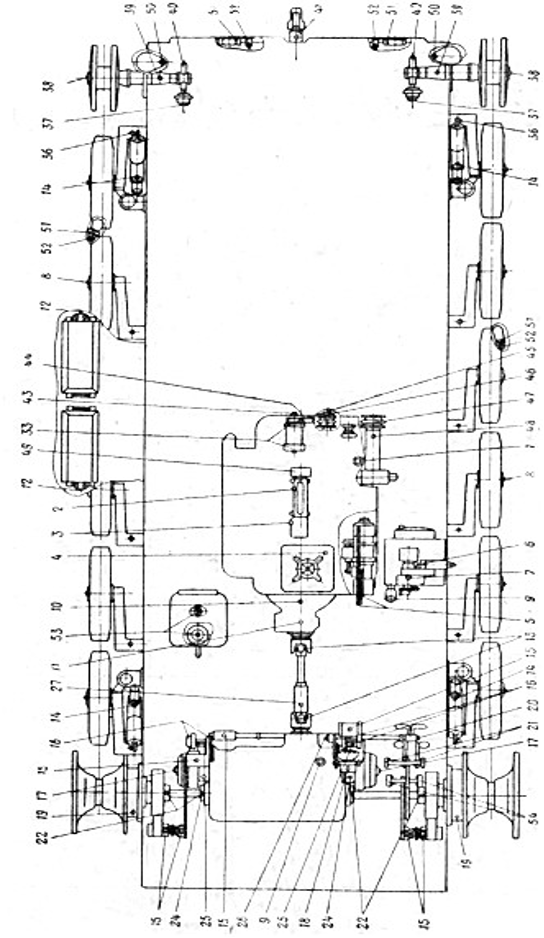
\includegraphics[height=0.95\textheight]{src/appendix_first.png}
    \caption{Схема смазки МТЛБ}
    \label{appendix_first}
\end{figure}


\begin{figure}
    \centering
    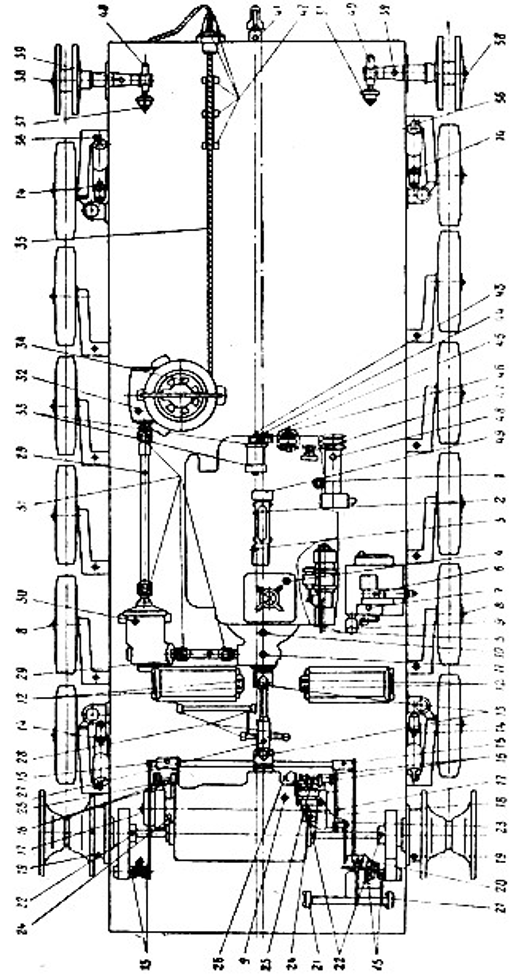
\includegraphics[height=0.95\textheight]{src/appendix_second.png}
    \caption{Схема смазки МТЛБ}
    \label{appendix_second}
\end{figure}

% Размеры колонок
\newcommand{\PointNumberSize}{1.1cm}
\newcommand{\PointNameSize}{1.8cm}
\newcommand{\PointCountSize}{1.53cm}
\newcommand{\TOSize}{1.5cm}
\newcommand{\AdditionalSize}{5cm}

\newcommand{\doublecolumn}[1]{\multicolumn{2}{m{\dimexpr \TOSize * 2 + 2\tabcolsep \relax}|}{#1}}
\newcommand{\triplecolumn}[1]{\multicolumn{3}{m{\dimexpr \TOSize * 3 + 4\tabcolsep \relax}|}{#1}}
\newcommand{\fullcolumn}[1]{\multicolumn{7}{>{\tc}m{\dimexpr \PointNumberSize + \PointNameSize + \PointCountSize + \TOSize * 3 + \AdditionalSize + 12\tabcolsep}}{\textbf{#1}}}

\newcommand{\doubleNameRaw}[1]{\multirow{2}{\PointNameSize}{\tc #1}}

\begin{scriptsize}
\begin{landscape}
\begin{longtable}{
    >{\tc}m{\PointNumberSize}|
    >{\tc}m{\PointNameSize}|
    >{\tc}m{\PointCountSize}|
    >{\tc}m{\TOSize}|
    >{\tc}m{\TOSize}|
    >{\tc}m{\TOSize}|
    m{\AdditionalSize}}

    \multirow{2}{\PointNumberSize}{\tc № точки смазки}  & \multirow{2}{\PointNameSize}{\tc Наименование точек смазок} &\multirow{2}{\PointCountSize}{\tc Количество точек смазок}   & \triplecolumn{\tc Техническое обслуживание} & \multirow{2}{\AdditionalSize}{\tc Дополнительные указания} \\
    \cline{4-6}
                    &   &  & ежедневное    &   №1    &   №2    & \\
    \hline\endhead
    \fullcolumn{\tc Масло Дс-11 (ГОСТ~8581-63), Дп-11 (ГОСТ~5304-54)~--- летом (при~температуре воздуха выше + 5°С),} \\
    \fullcolumn{\tc Дс-8 (ГОСТ~8581-63), Дп-8 (ГОСТ~5304-54)~--- зимой (при~температуре воздуха ниже + 5°C)} \\
    \hline
    \multirow{2}{*}{1} & \doubleNameRaw{Система смазки двигателя} & \multirow{2}{*}{1} & \triplecolumn{Проверить уровень масла в~картере двигателя, при~необходимости дозаправить} & При~дозаправке снять крышку с~заливной горловины, вставить воронку с~сеткой и~долить масло до~метки В на~щупе. \\
    & & & && Заменить масло & При~замене сразу~же после остановки двигателя слить масло из~картера двигателя и~масляного фильтра предварительной очистки. Промыть масляный фильтр налить масло в~поддон до~метки В на~щупе. \\
    \hline

    \multirow{2}{*}{2} & \doubleNameRaw{Топливный насос} & \multirow{2}{*}{1} & \triplecolumn{Проверить уровень масла в~корпусе топливного насоса, при~необходимости дозаправить} & При~дозаправке вывернуть пробку заливного отверстия и~долить масло до~верхней метки на~щупе.\\
    & & & && Через одно ТО-2 заменить масло & Заменить масло при~каждом снятии насоса с~двигателя \\
    \hline

    \multirow{2}{*}{3} & \doubleNameRaw{Картер регулятора топливного насоса} & \multirow{2}{*}{1} & \triplecolumn{Проверить уровень масла, при~необходимости дозаправить} & При~дозаправке вывернуть пробку заливного отверстия и~долить масло до~верхней метки на~щупе \\
    & & & && Через одно ТО-2 заменить масло & При~замене слить старое масло и~залить свежее до~требуемого уровня \\
    \hline
    
    5 & Подшип\-ники стартера & 3 & --- & --- & Через 500~ч работы двигателя или~при~ремонте смазать & Залить \range{10}{15} капель масла в~масленки стартера, в~средний и~задний подшипники залить по~30 капель масла \\ 
    \hline    \fullcolumn{Масло МТ-16л (ГОСТ~6360-58), летом и~зимой} \\
    \hline
    
    4 & Воздухо\-очиститель & 1 & \triplecolumn{Через \range{25}{30}~ч работы двигателя в~особо пыльных дорожных условиях. Через 50~ч в~условиях нормальной запыленности} & Фильтрующие кассеты тщательно промыть в~чистом дизельном топливе и~просушить. Две верхние кассеты пропитать маслом МТ-16п и~дать ему стечь до~прекращения каплепадения\\
    \hline
    
    \multirow{2}{*}{8} &  \doubleNameRaw{Подшип\-ники опорных катков} &  \multirow{2}{*}{12} & --- & \doublecolumn{Проверить уровень масла, при~необходимости дозаправить} & При~дозаправке вывернуть пробку контрольного отверстия и~долить масло \\
    & & & && Через одно ТО-2 заменить масло & При~замене вывернуть пробку сливного отверстия и~слить масло, промыть полость подшипников дизельным топливом и~залить свежее масло до~появления его из~контрольного отверстия. После преодоления водных препятствий проверить наличие воды в~масле, при~обнаружении следов воды масло заменить\\
    \hline
    
    \multirow{2}{*}{9} & \doubleNameRaw{ Главная передача и~масляный бак главной передачи} & \multirow{2}{*}{2} & --- & \doublecolumn{Проверить уровень масла, при~необходимости дозаправить} & При~дозаправке снять пробку заливной горловины масляного бака и~долить масло до~верхней зиговки заливной горловины \\
    & & & && Через одно ТО-2 заменить масло & При~замене слить масло из~масляного бака и~главной передачи сразу~же после остановки транспортера-тягача и~залить в~бак свежее масло до~верхней зиговки заливной горловины и~10~л в~главную передачу. Запустить двигатель, поработать \range{1}{2}~мин вхолостую и~при~необходимости дозаправить до~верхней зиговки заливной горловины бака. Масло МТ-4п (ГОСТ~6360-58) применять зимой в~районах эксплуатации с~особо низкими температурами воздуха (ниже $-$\celc{25}), а~также в~районах Крайнего Севера в~течение всего года \\
    \hline
    
    \multirow{2}{*}{11} & \doubleNameRaw{Промежу\-точный редуктор} & \multirow{2}{*}{1} & --- & \doublecolumn{Проверить уровень масла, при~необходимости дозаправить} & При~дозаправке вывернуть пробку и~долить масло до~уровня верхней метки на~щупе\\
    & & & && Через одно ТО-2 заменить масло & При~замене слить масло сразу~же после остановки транспортера-тягача и~залить свежее масло до~уровня верхней метки на~щупе \\
    \hline
    
    13 & Крестовины центрального карданного вала & 2 & --- & \doublecolumn{\tc Смазать} & Очистить масленку от~грязи и~нагнетать смазку до~появления свежей смазки из~предохранительного клапана\\ 
    \hline
    
    \multirow{2}{*}{19} &  \doubleNameRaw{Бортовые передачи} &  \multirow{2}{*}{2} & --- & \doublecolumn{Проверить уровень масла, при~необходимости дозаправить} & При~дозаправке вывернуть пробку контрольного отверстия и~долить масло до~уровня контрольного отверстия\\
    & & & && Через одно ТО-2 заменить масло & При~замене слить масло сразу~же после остановки транспортера-тягача и~залить свежее масло до~уровня контрольного отверстия. При~температуре ниже $-$\celc{30} применять масло МТ-14п (ГОСТ~6360-58). Заменители масла МТ-16п: летом~--- масло трансмиссионное автотракторное летнее; зимой~--- зимнее (ГОСТ~542-50) \\
    \hline
    
    30 & Реверс-редуктор лебедки & 1 & \triplecolumn{Через 100 подтягиваний и~50 спусков} & Вывернуть пробку и~долить масло до~уровня верхней метки на~щупе. Заменитель масла МТ-16п: масло АК-10 (ГОСТ~1862-63) летом и~зимой\\
    \hline
    
    31 & Крестовины карданов привода лебедки & 4 & \triplecolumn{Через 25 полных подтягиваний} & Рычажно-плунжерным шприцем с~насадкой нагнетать масло через крестовины кардана до~появления свежей смазки из~контрольного клапана. Заменители масла МТ-16п: летом~--- масло трансмиссионное автотракторное летнее, зимой~--- зимнее (ГОСТ~542-50)\\
    \hline
    
    32 & Лебедка & 1 &  \triplecolumn{Через 100 подтягиваний и~50 спусков} & Вывернуть пробку и~долить масло до~уровня верхней метки на~щупе. Заменитель масла МТ-16п: масло трансмиссионное автотракторное летнее~--- летом, зимнее~--- зимой (ГОСТ~542-50)\\
    \hline
    
    38 & Подшип\-ники направляющих колес & 2 & --- &  \doublecolumn{Проверить уровень масла, при~необходимости дозаправить} & При~дозаправке вывернуть пробку контрольного отверстия и~долить масло \\
    \hline
    
    \multirow{2}{*}{48} & \doubleNameRaw{Редуктор вентиля\-тора} & \multirow{2}{*}{1} & --- & \doublecolumn{Проверить уровень масла, при~необходимости дозаправить} & При~дозаправке отвернуть пробку со~щупом и~долить масло до~уровня метки на~щупе \\
    & & & && Заменить масло & При~замене отвернуть пробку, слить старое масло и~залить свежее до~уровня метки на~щупе \\
    \hline
    
    \newpage
    \fullcolumn{Смазка 1-13 жировая (ГОСТ~1631-61) или~ЦИАТИМ-201 (ГОСТ~6267-59) летом и~зимой} \\
    \hline

    10 & Муфта выключения главного фрикциона & 1 & \triplecolumn{\tc Смазать} & Очистить масленку и~заправить смазку, сделав \range{два}{три} нагнетания шприцем. При~движении в~тяжелых дорожных условиях при~частом переключении передач смазывать муфту ежедневно\\
    \hline
    
    16 & Подшип\-ники валиков кулаков мостиков управления & 4 & --- & --- & Через одно ТО-2 заменить смазку & Разобрать мостики управления, очистить подшипники от~старой смазки и~заложить новую. Заменитель смазки 1-13: консталин жировой УТ-1 (ГОСТ~1957-52) летом и~зимой\\
    \hline
    
    17 & Подшип\-ники ведущих барабанов фрикционов механизмов поворота & 2 & \triplecolumn{\tc Смазать} & Очистить масленку от~грязи и~сделать \range{пять}{шесть} нагнетаний шприцем. Заменитель смазки 1-13: консталин жировой УТ-1 (ГОСТ~1957-52) летом и~зимой\\
    \hline

    18 & Колонка переключения передач & 2 & \triplecolumn{\tc Смазать} & Очистить масленку от~грязи и~нагнетать до~появления свежей смазки из-под поводков. Заменитель смазки 1-13: консталин жировой УТ-1 (ГОСТ~1957-52) летом и~зимой\\
    \hline
    
    22 & Шлицевые соединения зубчатых карданов главной передачи & 4 & \triplecolumn{\tc Смазать} & Очистить масленку от~грязи и~нагнетать до~появления свежей смазки из-под уплотнений. \\
    \hline
    
    24 & Подшип\-ники механизмов выключения фрикционов и~механизмов поворота & 2 & \triplecolumn{\tc Смазать} & Очистить масленку от~грязи и~нагнетать до~появления свежей смазки из-под колец. При~движении на~плаву заправлять ежедневно. Заменитель смазки 1-13: консталин жировой УТ-1 (ГОСТ~1957-52) летом и~зимой\\
    \hline
    
    25 & Мостики управления & 2 & \triplecolumn{\tc Смазать} & Очистить масленку от~грязи и~сделать \range{пять}{шесть} нагнетаний шприцем. Заменитель смазки 1-13: консталин жировой УТ-1 (ГОСТ~1957-52) летом и~зимой\\
    \hline
    
    43 & Подшип\-ники шкива привода компрессора & 1 & --- & --- & Смазать & Очистить масленку от~грязи и~сделать \range{три}{четыре} нагнетания шприцем\\ 
    \hline
    
    44 & Подшип\-ники натяжного ролика привода генератора & 2 & \triplecolumn{\tc Смазать} & Очистить масленку от~грязи сделать \range{три}{четыре} нагнетания шприцем. Заменитель смазки 1-13: консталин жировой УТ-1 (ГОСТ~1957-52) летом и~зимой\\
    \hline

    45 & Подшип\-ники натяжного ролика привода компрессора & 1 & --- & --- & Смазать & Очистить масленку от~грязи и~сделать \range{четыре}{пять} нагнетаний шприцем\\ 
    \hline
    
    46 & Подшип\-ники натяжного ролика ремня вентилятора & 1 & \triplecolumn{\tc Смазать} & Очистить масленку от~грязи и~сделать \range{пять}{шесть} нагнетаний шприцем. Заменитель смазки 1-13: консталин жировой УТ-1 (ГОСТ~1957-52) летом и~зимой\\
    \hline
    
    47 & Подшип\-ники водяного насоса & 1 & --- & \doublecolumn{\tc Смазать} & Очистить масленку от~грязи и~нагнетать до~появления свежей смазки из~верхнего контрольного отверстия\\ 
    \hline    \fullcolumn{Солидол синтетический (ГОСТ~4366-64) летом и~зимой} \\
    \hline

    12 & Клеммы аккумуляторных батарей & 4 & --- & \doublecolumn{\tc Смазать} & Клеммы очистить от~окиси, закрепить на~них провода и~смазать клеммовые соединения \\
    \hline
    
    20 & Валик рычагов управления & 1 & --- & \doublecolumn{\tc Смазать} & Очистить масленку от~грязи и~нагнетать до~появления свежей смазки в~торцах кронштейна\\
    \hline
    
    23 & Переходный валик тяги левого мостика управления & 1 & --- & --- & Смазать & То~же\\
    \hline
    
    26 & Валик тяги главного фрикциона & 1 & --- & --- & Смазать & То~же\\
    \hline
    
    36 & Кронштей\-ны подвески & 12 & --- & --- & Смазать & Вывернуть пробку, ввернуть шланг и~сделать \range{два}{три} нагнетания шприцем\\
    \hline

    37 & Подшип\-ники натяжных винтов направляющих колес & 2 & --- & \doublecolumn{\tc Смазать} & Очистить масленку от~грязи и~сделать \range{три}{четыре} нагнетания шприцем \\
    \hline

    40 & Натяжные винты направляющих колес & 2 & --- & \doublecolumn{\tc Смазать} & Очистить винт от~грязи и~смазать \\
    \hline

    41 & Тягово-сцепной прибор & 1 & --- & \doublecolumn{\tc Смазать} & Очистить масленку от~грязи и~сделать \range{пять}{шесть} нагнетаний шприцем\\
    \hline

    15 & Подшип\-ники передаточного вала и~кронштейнов остановочных тормозов & 6 на~МТЛ, 7~на~МТ-ЛБ & --- & --- & Смазать & Очистить масленку от~грязи и~сделать \range{три}{четыре} нагнетания шприцем\\
    \hline

    52 & Механизмы запирания бортовых лючков & 4 & --- & --- & Заменить смазку & Разобрать механизм запирания бортовых лючков, удалить старую смазку и~заложить новую \\
    \hline

    51 & Шаровые опоры бортовых лючков & 4 & --- & --- & Заменить смазку & Разобрать шаровую опору бортовых лючков, удалить старую смазку и~заложить новую \\
    \hline
    
    50 & Механизмы запирания крышек заливных горловин топливных баков & 2 & --- & --- & Заменить смазку & Разобрать механизм запирания крышек заливных горловин, удалить старую смазку и~заложить новую\\
    \hline

    39 & Кронштейн направляющих колес & 2 & --- & --- & Через одно ТО-2 смазать & Очистить масленку от~грязи и~сделать \range{15}{20} нагнетаний шприцем\\
    \hline

    27 & Шлицевое соединение центрального карданного вала & 1 & --- & --- & Через одно ТО-2 смазать & Разобрать шлицевое соединение карданного вала, удалить старую смазку и~заложить новую\\
    \hline

    21 & Подшипники валика педали главного фрикциона & 2 & --- & --- & Через одно ТО-2 заменить смазку & Разобрать валик педали главного фрикциона, очистить подшипники от~старой смазки и~заложить новую\\
    \hline

    54 & Подшипники промежуточного вала левого рычага управления & 2 & --- & --- & Через одно ТО-2 заменить смазку & Разобрать промежуточный вал, очистить подшипники от~старой смазки и~заложить новую\\
    \hline
    
    53 & Сиденье поворотное & 2 & --- & --- & Через одно ТО-2 заменить смазку & Снять сиденье, очистить полости кронштейнов от~старой смазки и~заполнить новой смазкой \\
    \hline
    
    29 & Шлицевые соединения карданных валов привода лебедки & 2 & \triplecolumn{Через 100 полных подтягиваний и~50 спусков смазать} & Очистить масленки от~грязи и~сделать \range{пять}{шесть} нагнетаний шприцем\\
    \hline
    
    42 & Датчик ограничителя усилия на~тросе лебедки и~выводное устройство троса лебедки & 5 & \triplecolumn{Через \range{20}{25} полных подтягиваний смазать} & Очистить масленки от~грязи и~сделать \range{три}{четыре} нагнетания шприцем\\
    \hline
    
    34 & Подшипники ступицы барабана лебедки & 1 & \triplecolumn{Через \range{20}{25} полных подтягиваний смазать} & Очистить масленки от~грязи и~сделать \range{три}{четыре} нагнетания шприцем\\
    \hline
    
    28 & Подшипники валиков привода управления лебедкой & 4 & \triplecolumn{Через 100 полных подтягиваний и~50 спусков смазать} & Разобрать привод, удалить старую смазку и~заполнить новой \\
    \hline
    
    35 & Трос лебедки & 1 & \triplecolumn{Каждый раз при~пользовании лебедкой смазать} &  После окончания работы очистить трос от~грязи и~при~наматывании на~барабан смазать\\
    \hline

    \fullcolumn{Смазка ЦИАТИМ-203 (ГОСТ~8773-63)}\\
    \hline

    49 & Муфта опережения впрыска топлива & 1 & \triplecolumn{При~ремонте муфты заменить смазку} & После разборки муфты удалить старую смазку и~заложить новую\\
    \hline

    \fullcolumn{Смазка Л3-158 (ВТУ ТН3 №100-61), ЦИАТИМ-221 (ГОСТ~9433-60) или~ЦИАТИМ-201 (ГОСТ~6267-59)} \\
    \hline

    33 & Подшипники генератора & 2 & --- & --- & Через 1000~ч работы двигателя заменить смазку & Снять генератор с~двигателя, разобрать его, удалить старую смазку и~промыть шарикоподшипники в~бензине. Заложить в~подшипники свежую смазку. Собрать генератор и~установить на~двигатель\\
    \hline    \fullcolumn{Смесь из~50\% трансформаторного масла (ГОСТ~982-68) и~50\% турбинного масла (ГОСТ~32-53)}\\
    \hline

    14 & Гидроамор\-тизаторы & 4 & --- & --- & Дозаправить & Дозаправить гидроамортизатор без~его снятия. Очистить гидроамортизатор от~грязи, отвернуть пробку компенсационной камеры и~линейкой проверить уровень жидкости. Расстояние от~дна компенсационной камеры до~уровня жидкости должно быть: 
    \begin{itemize}
        \item при~загруженном транспорте~--- \range{140}{150}~\textit{мм};
        \item при~разгруженном транспорте: 
            \begin{itemize}
            \item передние \range{148}{154} \textit{мм};
            \item задние  \range{128}{132} \textit{мм}.
            \end{itemize}
    \end{itemize}\\
    \hline
    
    \fullcolumn{Смесь из~70\% масла дизельного Дс-8 (ГОСТ~8581-63) с~присадкой и~30\% дизельного топлива (ГОСТ~4749-49) марки ДЗ, летом и~зимой}\\
    \hline 

    6 & Редуктор подогревателя & 1 & \triplecolumn{Через \range{10}{15}~ч работы редуктора или~через \range{20}{30} пусков дозаправить (при~очередном ТО-1)} & Отвернуть пробку заливного и~контрольного отверстия залить смесь до~уровня контрольного отверстия\\
    \hline 

    7 & Опора верхнего валика редуктора подогревателя & 1 & \triplecolumn{Через \range{10}{15}~ч работы редуктора или~через \range{20}{30} пусков дозаправить (при~очередном ТО-1)} & Отвернуть пробку и~залить \range{2}{3}~см$^3$ смеси\\
    \hline

\end{longtable}
\end{landscape}
\end{scriptsize}
